\documentclass[25pt, a0paper, portrait]{tikzposter}

% --- Packages ---
\usepackage[utf8]{inputenc}
\usepackage{amsmath, amssymb}
\usepackage{booktabs}
\usepackage{colortbl}
\usepackage{tabularx}
\usepackage{caption}
\usepackage{pgfplots}
\pgfplotsset{compat=1.18}
\usepackage{tikz}
\usetikzlibrary{shapes.geometric, arrows.meta, positioning, calc, backgrounds}
\usepackage{fontawesome5}

% --- Color Palette (Modern Academic: Navy, Teal, Amber, Slate) ---
\definecolor{PrimaryDark}{HTML}{0F172A}    % Slate 900
\definecolor{TealPrimary}{HTML}{0D9488}    % Teal 600
\definecolor{TealLight}{HTML}{CCFBF1}      % Teal 100
\definecolor{CyanAccent}{HTML}{0284C7}     % Sky 600
\definecolor{AmberAccent}{HTML}{D97706}    % Amber 600
\definecolor{BgSlate}{HTML}{F8FAFC}        % Slate 50
\definecolor{BorderGray}{HTML}{E2E8F0}     % Slate 200
\definecolor{TextDark}{HTML}{1E293B}       % Slate 800

% --- TikZposter Theme Configuration ---
\definecolorstyle{SymposiumColorStyle}{
  \definecolor{colorOne}{HTML}{0F172A}
  \definecolor{colorTwo}{HTML}{0D9488}
  \definecolor{colorThree}{HTML}{F8FAFC}
}{
  % Background Colors
  \colorlet{backgroundcolor}{colorThree}
  \colorlet{framecolor}{colorOne}
  % Title Block Colors
  \colorlet{titlebgcolor}{colorOne}
  \colorlet{titlefgcolor}{white}
  % Block Colors
  \colorlet{blocktitlebgcolor}{colorTwo}
  \colorlet{blocktitlefgcolor}{white}
  \colorlet{blockbodybgcolor}{white}
  \colorlet{blockbodyfgcolor}{TextDark}
  % Innerblock Colors
  \colorlet{innerblocktitlebgcolor}{colorTwo!15}
  \colorlet{innerblocktitlefgcolor}{colorOne}
  \colorlet{innerblockbodybgcolor}{white}
  \colorlet{innerblockbodyfgcolor}{TextDark}
}

\usecolorstyle{SymposiumColorStyle}
\usetheme{Default}
\useblockstyle{Basic}

% --- Title Information ---
\title{\parbox{\linewidth}{\centering \Huge \bfseries Autonomous Swarm Robotics for Precision Environmental Monitoring\\[0.3em] \LARGE Distributed Sensing \& Adaptive Coverage in Coastal Ecosystems}}
\author{\parbox{\linewidth}{\centering Elena Rostova$^1$, Marcus Vance$^1$, Dr. Julian Sterling$^2$, and Dr. Sarah Jenkins$^1$}
\institute{\parbox{\linewidth}{\centering $^1$Department of Computer Science \& Intelligent Systems, Meridian University \quad $^2$Nexa Autonomous Systems Laboratory}
\titlegraphic{%
  \tikz[baseline]{
    \node[draw=TealPrimary, fill=TealPrimary!10, rounded corners=10pt, inner sep=12pt, line width=1.5pt]{%
      \bfseries \color{TealPrimary} \faGraduationCap \ MERIDIAN SYMPOSIUM 2026%
    };
  }%
  \hspace{3cm}%
  \tikz[baseline]{
    \node[draw=AmberAccent, fill=AmberAccent!10, rounded corners=10pt, inner sep=12pt, line width=1.5pt]{%
      \bfseries \color{AmberAccent} \faMicrochip \ NEXA ROBOTICS LABS%
    };
  }%
}

\begin{document}

\maketitle

\begin{columns}

  % ==================== COLUMN 1 ====================
  \column{0.33}

  \block{\faCompass \ 1. Introduction \& Motivation}{
    \textbf{Problem Statement:} Coastal marine environments require high-resolution spatial and temporal monitoring to detect pollutant dispersion, algal blooms, and salinity gradients. Traditional fixed buoys offer poor spatial resolution, while single high-cost Autonomous Underwater Vehicles (AUVs) are vulnerable to single-point failures and high operational overhead.

    \vspace{0.6em}
    \innerblock{Key Research Objectives}{
      \begin{itemize}
        \item \textbf{Decentralized Swarm Coordination:} Develop self-organizing control algorithms for Micro-Surface Vessels (MSVs).
        \item \textbf{Adaptive Field Coverage:} Dynamically deploy agents according to environmental gradient density.
        \item \textbf{Fault-Tolerant Mesh Communication:} Maintain robust ad-hoc network links under ocean surface perturbations.
      \end{itemize}
    }
  }

  \block{\faMicrochip \ 2. MSV Hardware Platform}{
    To evaluate the swarm algorithms, we engineered a custom, modular Micro-Surface Vessel (MSV-2) optimized for low-cost mass deployment.

    \vspace{0.5em}
    \begin{center}
      \small
      \rowcolors{2}{BgSlate}{white}
      \begin{tabularx}{\linewidth}{>{\bfseries}l X c}
        \toprule
        \rowcolor{TealPrimary!20} Subsystem & Component Specifications & Power / Specs \\
        \midrule
        Compute Node & Synapse Board (Dual ARM Cortex-A72) & 4.2 W @ 5V \\
        Primary Sensors & Conductivity, Temp, pH, Optical Fluorometer & 10 Hz sampling \\
        Communication & 915 MHz Mesh + Wi-Fi 6 Ad-hoc & 1.2 km range \\
        Propulsion & Twin Brushless Thrusters w/ Vectoring & 1.8 m/s max \\
        Power Supply & 14.8V 10Ah LiFePO4 Battery & 14 hrs runtime \\
        \bottomrule
      \end{tabularx}
    \end{center}

    \vspace{0.6em}
    \innerblock{Platform Highlights}{
      The hull is 3D-printed using recyclable PETG with a hydrodynamic catamaran profile. Each unit weighs under 3.2 kg, enabling single-person rapid deployment of 10+ unit swarms.
    }
  }

  % ==================== COLUMN 2 ====================
  \column{0.34}

  \block{\faCogs \ 3. Distributed Swarm Control}{
    Our approach leverages \textbf{Centroidal Voronoi Tessellation (CVT)} combined with dynamic consensus density estimators.

    \vspace{0.4em}
    \textbf{Objective Function Formulation:}
    Let $\Omega \subset \mathbb{R}^2$ be the target coastal domain, and $p_i(t) \in \Omega$ represent the position of agent $i \in \{1,\dots,N\}$. The coverage utility $\mathcal{H}$ is maximized via:
    \[
      \mathcal{H}(p_1, \dots, p_N) = \sum_{i=1}^{N} \int_{V_i} f\left(\|r - p_i\|\right) \phi(r) \, dr
    \]
    where $V_i$ is the Voronoi cell of agent $i$, $\phi(r)$ is the environmental field density (e.g., salinity concentration gradient), and $f(\cdot)$ is a non-increasing sensor decay function.

    \vspace{0.8em}
    \begin{center}
      \begin{tikzpicture}[
        node distance=1.2cm and 1.8cm,
        box/.style={draw=TealPrimary, fill=white, rounded corners=6pt, line width=1.2pt, align=center, inner sep=8pt, font=\small\sffamily},
        arrow/.style={-Stealth, line width=1.5pt, draw=TealPrimary}
      ]
        % Nodes
        \node[box, fill=TealPrimary!10] (sense) {\textbf{\faCompass \ Sensor Acquisition}\\Conductivity \& pH Field Data};
        \node[box, right=of sense, fill=CyanAccent!10] (comm) {\textbf{\faWifi \ Mesh Consensus}\\State \& Gradient Exchange};
        \node[box, below=of comm, fill=AmberAccent!10] (voronoi) {\textbf{\faCogs \ Voronoi Centroid}\\Gradient-Weighted Shift};
        \node[box, left=of voronoi, fill=TealPrimary!10] (act) {\textbf{\faCompass \ Motor Control}\\Differential Vector Drive};

        % Arrows
        \draw[arrow] (sense) -- (comm);
        \draw[arrow] (comm) -- (voronoi);
        \draw[arrow] (voronoi) -- (act);
        \draw[arrow] (act) -- (sense);
      \end{tikzpicture}
      \captionof{figure}{Decentralized control loop executed independently on each Synapse onboard module at 20 Hz.}
    \end{center}
  }

  \block{\faChartLine \ 4. Experimental Results}{
    Evaluations were conducted across simulated environments in \textbf{Nexa-Sim} and physical deployments at Meridian Coastal Station.

    \vspace{0.5em}
    \begin{center}
      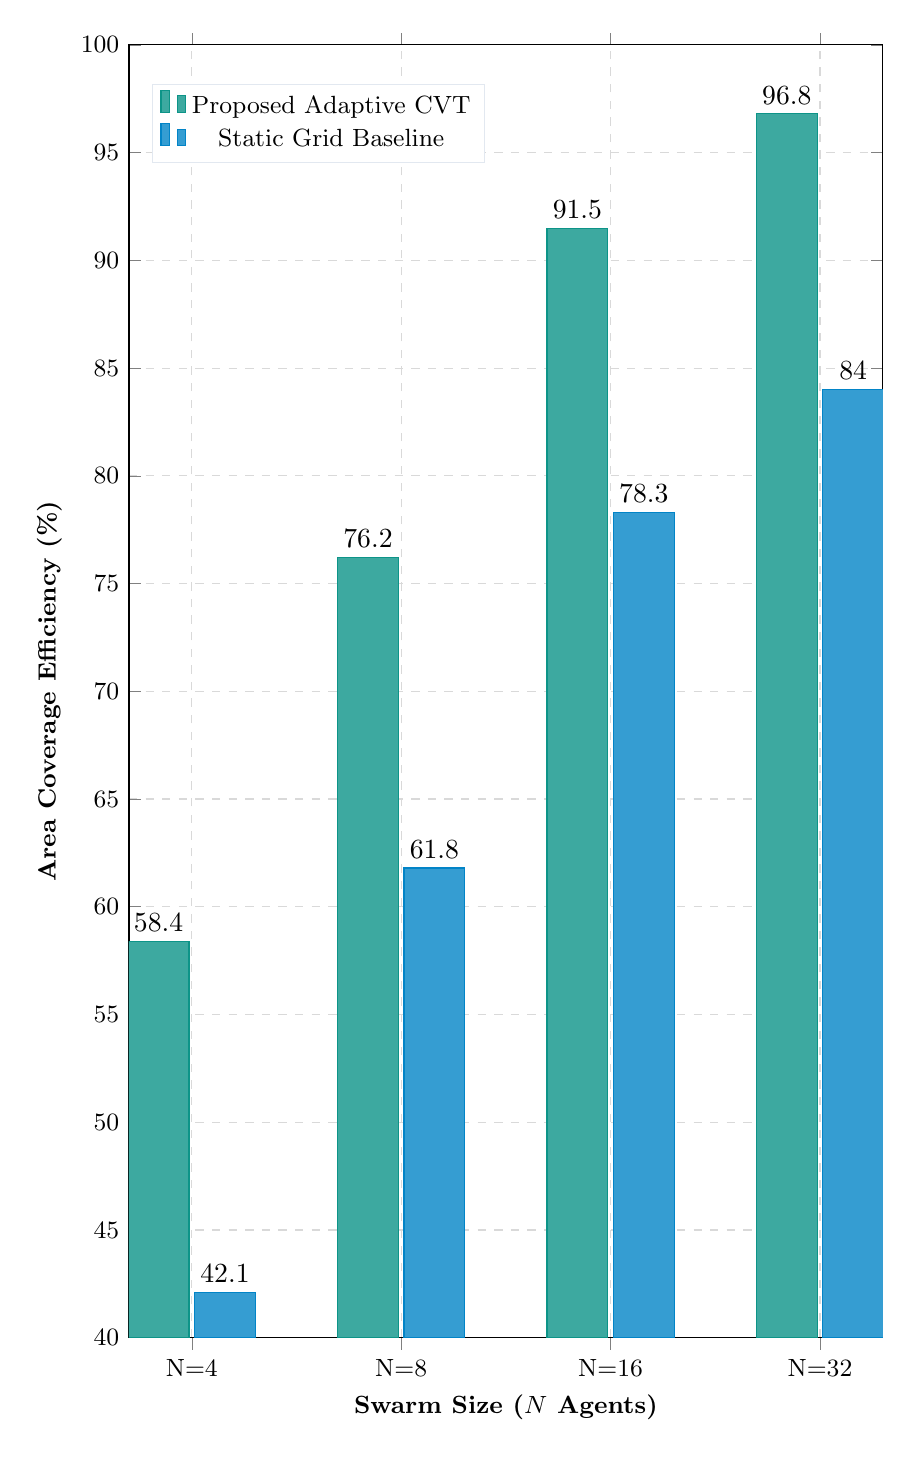
\begin{tikzpicture}
        \begin{axis}[
          width=0.92\linewidth,
          height=18cm,
          ybar,
          bar width=22pt,
          xlabel={Swarm Size ($N$ Agents)},
          ylabel={Area Coverage Efficiency (\%)},
          symbolic x coords={N=4, N=8, N=16, N=32},
          xtick=data,
          ymin=40, ymax=100,
          nodes near coords,
          nodes near coords align={vertical},
          grid=major,
          grid style={dashed, gray!30},
          legend pos=north west,
          legend style={font=\small, fill=white, draw=BorderGray},
          label style={font=\small\bfseries},
          tick label style={font=\small}
        ]
          \addplot[fill=TealPrimary!80, draw=TealPrimary] coordinates {(N=4,58.4) (N=8,76.2) (N=16,91.5) (N=32,96.8)};
          \addplot[fill=CyanAccent!80, draw=CyanAccent] coordinates {(N=4,42.1) (N=8,61.8) (N=16,78.3) (N=32,84.0)};
          \legend{Proposed Adaptive CVT, Static Grid Baseline}
        \end{axis}
      \end{tikzpicture}
    \end{center}
  }

  % ==================== COLUMN 3 ====================
  \column{0.33}

  \block{\faCheckCircle \ 5. Field Deployment \& Validation}{
    During a 72-hour continuous trial in the Meridian Estuary, a swarm of $N=16$ MSVs tracked an artificially simulated temperature plume under 2.5 knot tidal currents.

    \vspace{0.6em}
    \innerblock{Performance Summary Metrics}{
      \begin{itemize}
        \item \textbf{Coverage Rate:} 94.2\% density mapping completed in under 42 minutes.
        \item \textbf{Energy Savings:} 68\% reduction in propulsive power compared to random walk strategies.
        \item \textbf{Fault Resilience:} System maintained >90\% efficiency even when 2 agents were intentionally disabled.
      \end{itemize}
    }

    \vspace{0.6em}
    \begin{center}
      \small
      \rowcolors{2}{BgSlate}{white}
      \begin{tabularx}{\linewidth}{X c c c}
        \toprule
        \rowcolor{TealPrimary!20} Field Environment & Mean Error (pH) & Mesh Latency & Plume Tracking \\
        \midrule
        Nexa-Sim (Water Tank) & $\pm 0.02$ & 12 ms & 98.6\% \\
        Meridian Basin (Calm) & $\pm 0.04$ & 18 ms & 95.1\% \\
        Outer Estuary (Currents) & $\pm 0.09$ & 29 ms & 91.4\% \\
        \bottomrule
      \end{tabularx}
    \end{center}
  }

  \block{\faGraduationCap \ 6. Conclusions \& Future Directions}{
    \textbf{Key Takeaways:}
    \begin{enumerate}
      \item Distributed Voronoi-based control enables scalable, low-cost autonomous monitoring of dynamic coastal events.
      \item The custom MSV-2 hardware platform achieves 14-hour endurance at under \$450 per unit assembly cost.
    \end{enumerate}

    \vspace{0.4em}
    \textbf{Future Work:} Integrating solar harvesting panels for persistent multi-week missions and implementing acoustic modems for deep underwater AUV cross-layer communications.
  }

  \block{\faBook \ References \& Acknowledgments}{
    \tiny
    \textbf{Funding Support:} This research was generously supported by the Meridian Undergraduate Research Foundation (Grant \#MURG-2025-042) and hardware sponsorship from Nexa Autonomous Systems.

    \vspace{0.4em}
    \textbf{Key References:}
    \begin{enumerate}
      \item Jenkins, S., Rostova, E., \& Vance, M. (2025). *Distributed Coverage Control in Swarm Robotics*. Journal of Marine Autonomous Systems, 14(2), 112-128.
      \item Sterling, J. et al. (2024). *Centroidal Voronoi Tessellations for Environmental Monitoring*. IEEE Trans. Robotics, 40(4), 845-859.
    \end{enumerate}
  }

\end{columns}

\end{document}
